\section{System Design}
\label{sec:system_design}
In this section we describe the system design as a hardware/software co-design framework for floating-point CNN acceleration targeting resource-limited FPGAs. This is a scalable and parameterized architecture that allows design exploration integrated with TensorFlow Lite.

\subsection{Base embedded system architecture} As a hardware/software co-design, the system architecture is an embedded CPU+FPGA-based platform, where the acceleration of tensor operations is based on asynchronous\footnote{The system is synchronous at the circuit level, but the execution is asynchronous in terms of jobs.} execution in parallel TPs. \Fig{fig:system_architecture} illustrates the system hardware architecture as a scalable structure. For operational configuration, each TP uses AXI-Lite interface. For data transfer, each TP uses AXI-Stream interfaces via Direct Memory Access (DMA) allowing data movement with high transfer rate. Each TP asserts an interrupt flag once the job or transaction is complete. Interrupt events are handled by the embedded CPU to collect results and start a new transaction.

The hardware architecture can resize its resource utilization by modifying the number of TP instances prior to the hardware synthesis, this provides scalability with a good trade-off between area and throughput.
\begin{figure}[t!]
	\centering
	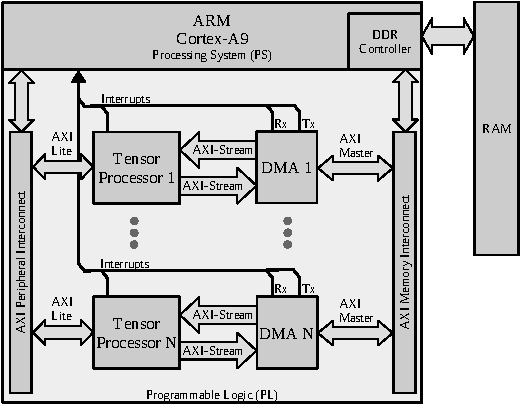
\includegraphics[width=0.5\textwidth]{../figures/system_design.pdf}
	\caption{Base embedded system architecture.}
	\label{fig:system_architecture}
\end{figure}
\subsection{Tensor processor}
The TP is a dedicated hardware module to compute tensor operations. The hardware architecture is described in \fig{fig:accelerator}. This architecture implements high performance off-chip communication with AXI-Stream, direct CPU communication with AXI-Lite, and on-chip storage utilizing BRAM. This hardware architecture is implemented with high-level synthesis (HLS). The tensor operations are implemented based on the C++ TensorFlow Lite micro kernels.
\begin{figure}[t!]
	\centering
	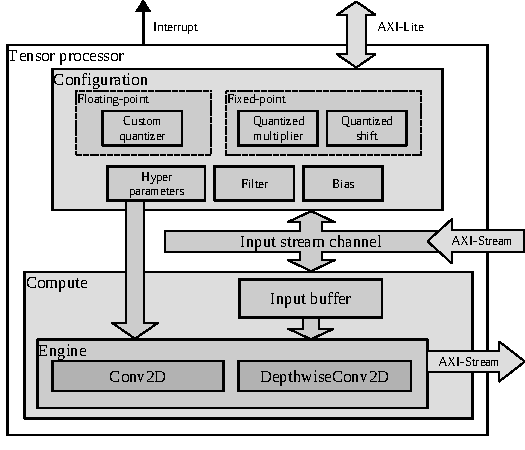
\includegraphics[width=0.5\textwidth]{../figures/accelerator.pdf}
	\caption{Hardware architecture of the proposed tensor processor.}
	\label{fig:accelerator}
\end{figure}
\subsubsection{\textbf{Modes of operation}} This accelerator offers two modes of operation: \emph{configuration} and \emph{execution}.
\begin{itemize}
	\item In \emph{configuration} mode, the TP receives the tensor operation ID and hyperparameters: stride, dilation, padding, offset, activation, depth-multiplier, input shape, filter shape, bias shape, and output shape. Afterwards, the TP receives filter and bias tensors to be locally stored.
	
	\item In \emph{execution} mode, the TP executes the tensor operator according to the hyperparameters given in the configuration mode. During execution, the input and output tensor-buffers are moved from/to the TF Lite memory regions via DMA.
\end{itemize}
\subsubsection{\textbf{Dot-product with with hybrid custom
		floating-point and logarithmic
		dot-product approximation}}
\label{sec:dot_product}
We optimize the floating-point computation adopting the dot-product with hybrid custom floating-point and logarithmic approximation\cite{nevarez2021accelerating}. The hardware dot-product is illustrated in \Fig{fig:dot_product}. This approach: (1) denormalizes input values, (2) executes computation with integer format for exponent and mantissa, and finally, (3) it normalizes the result into IEEE 754 format, see \Fig{fig:dot_product_hybrid}. Rather than a parallelized structure, this is a pipelined hardware design suitable for resource-limited devices. The latency in clock cycles of this hardware module is defined by \equ{eq:dot_custom_float_latency} and \equ{eq:dot_log_latency}, where $N$ is the dot-product vector length. The latency equations are obtained from the general pipelined hardware latency formula: $L=\left(N-1\right)II+IL$, where $II$ is the initiation interval (\fig{fig:dot_product_hybrid}(a)), and $IL$ is the iteration latency (\fig{fig:dot_product_hybrid}(b)). Both $II$ and $IL$ are obtained from the high-level synthesis analysis. The logarithmic approximation removes the mantissa bit-field, which removes the mantissa multiplication and correction in clock cycle 3 and 4, respectively, see \fig{fig:dot_product_hybrid}.
\begin{eqnarray} \label{eq:dot_custom_float_latency}
L_{custom}=N+7
\end{eqnarray}
\begin{eqnarray} \label{eq:dot_log_latency}
L_{log}=N+6
\end{eqnarray}
 As a design parameter, both the exponent and mantissa bit-width of the weight/filter vector provides a tunable knob to trade-off between resource utilization and QoR \cite{park2009dynamic}. These parameters must be defined before hardware synthesis.
\begin{figure}[t!]
	\centering
	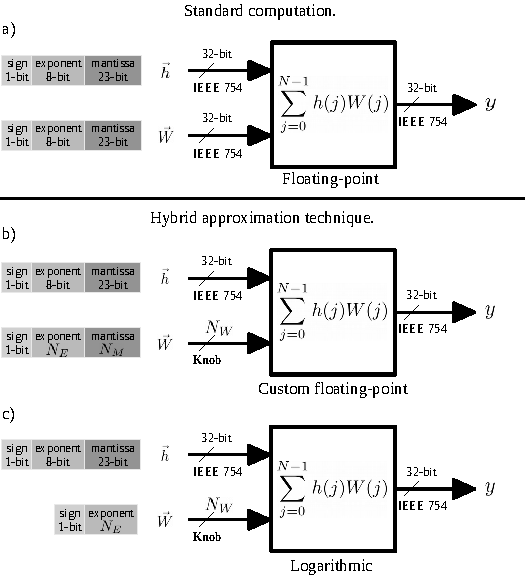
\includegraphics[width=0.5\textwidth]{../figures/dot-product_unit.pdf}
	\caption{Dot-product hardware module with (a) standard floating-point
		(IEEE 754) arithmetic, (b) hybrid custom floating-point, and (c) hybrid logarithmic approximation.}
	\label{fig:dot_product}
\end{figure}
\begin{figure}[t!]
	\centering
	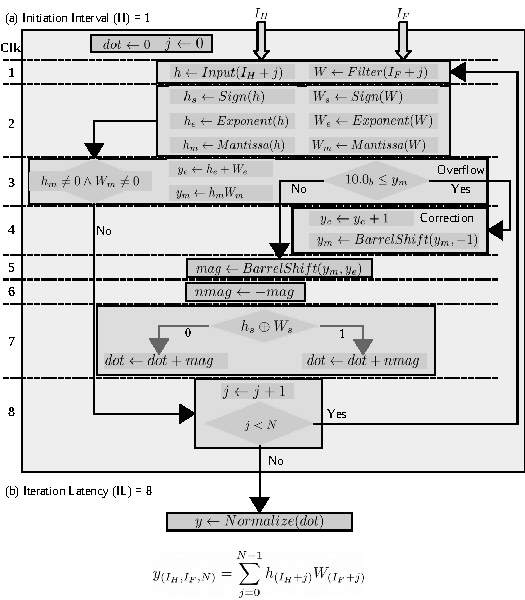
\includegraphics[width=0.5\textwidth]{../figures/dot_product_hybrid.pdf}
	\caption{Pipelined hardware module for vector dot-product with hybrid custom floating-point, (a) exhibits the initiation interval of 1 clock cycle, and (b) presents
		the iteration latency of 8 clock cycles. $I_H$ and $I_F$ represent the input and filter buffer indexes, respectively.}
	\label{fig:dot_product_hybrid}
\end{figure}
\subsubsection{\textbf{On-chip memory utilization}}
The total on-chip memory utilization on the TP is defined by \Equ{eq:tp_memory}, where $Input_{M}$ is the \emph{input buffer}, $Filter_{M}$ is the \emph{filter buffer}, $Bias_{M}$ is the \emph{bias buffer}, and $V_{M}$ represents the local variables required for operation. The on-chip memory buffers are defined in bits. \fig{fig:accelerator} illustrates the convolution operation utilizing the on-chip memory buffers.
\begin{figure}[t!]
	\centering
	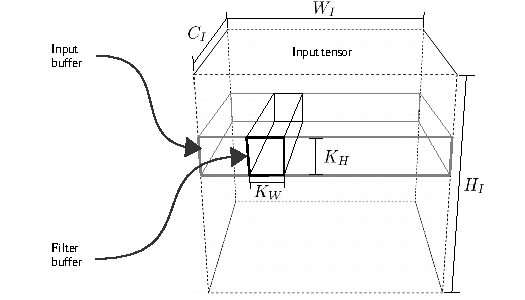
\includegraphics[width=0.5\textwidth]{../figures/accelerator_buffers.pdf}
	\caption{Design parameters for on-chip memory buffers on the TP.}
	\label{fig:accelerator_buffers}
\end{figure}
\begin{eqnarray} \label{eq:tp_memory}
TP_{M}=Input_{M}+Filter_{M}+Bias_{M}+V_{M}
\end{eqnarray}
The memory utilization of \emph{input buffer} is defined by \Equ{eq:input_memory}, where $K_{H}$ is the height of the convolution kernel, $W_{I}$ is the width of the input tensor, $C_{I}$ is the number of input channels, and $BitSize_{I}$ is the bit size of each input tensor element.
\begin{eqnarray} \label{eq:input_memory}
Input_{M}=K_{H}W_{I}C_{I}BitSize_{I}
\end{eqnarray}
The memory utilization of \emph{filter buffer} is defined by \Equ{eq:filter_memory}, where $K_{W}$ and $K_{H}$ are the width and height of the convolution kernel, respectively; $C_{I}$ and $C_{O}$ are the number of input and output channels, respectively; and $BitSize_{F}$ is the bit size of each filter element.
\begin{eqnarray} \label{eq:filter_memory}
Filter_{M}=C_{I}K_{W}K_{H}C_{O}BitSize_{F}
\end{eqnarray}
The memory utilization of \emph{bias buffer} is defined by \Equ{eq:bias_memory}, where $C_{O}$ is the number of output channels, and $BitSize_{B}$ is the bit size of each bias element.
\begin{eqnarray} \label{eq:bias_memory}
Bias_{M}=C_{O}BitSize_{B}
\end{eqnarray}
As a design trade-off, \Equ{eq:channel_in_memory} defines the capacity of output channels based on the given design parameters. The total on-chip memory $TP_{M}$ determines the TP capacity.
\begin{eqnarray} \label{eq:channel_in_memory}
C_{O}=\frac{TP_{M}-V_{M}-K_{H}W_{I}C_{I}BitSize_{I}}{C_{I}K_{W}K_{H}BitSize_{F}+BitSize_{B}}
\end{eqnarray}
The number formats implemented in the TP are defined by $BitSize_F$, $BitSize_B$ and $BitSize_I$. For example, a 5-bit custom floating-point format can be defined by 1-bit sign, 3-bit exponent and 1-bit mantissa. These are design parameters defined before hardware synthesis. This allows fine control of BRAM utilization, suitable for resource-limited devices.

\subsection{Quantized aware training}
The quantize-aware training method is an iterative optimization. The custom CNN model is initially trained with early stop monitoring until minimal validation loss, then the CNN model is retrained including the quantization method implemented as a callback function on every batch end, see \Algo{alg:training}. The quantization method maps the full precision filter and bias values to the closest representable quantized values, see \Algo{alg:quantize_training}. The quantize-aware training method starts with a wide exponent size target (e.g. 5-bits) and gradually reduces the target size until the model drops to a given accuracy degradation threshold (e.g. 1\%). We have observed that the exponent bit size plays a more predominant influence on the model accuracy than the mantissa bit size. The mantissa bit size can be set to the minimum (e.g. 1-bit). This method quantizes the filter and bias tensors of the \emph{Conv2D} and \emph{SeparableConv2D} layers. This method is integrated in TensorFlow/Keras framework. The resulting quantized parameters are truncated and buffered in the on-chip memory of the TP during \emph{configuration} mode.
\begin{algorithm}[h!]
	\label{alg:training}
	\caption{Training method.}
	\begin{algorithmic}
		\SetAlgoLined
		\renewcommand{\algorithmicrequire}{\textbf{input:}}
		\renewcommand{\algorithmicensure}{\textbf{output:}}
		\REQUIRE $MODEL$ as the CNN.
		\REQUIRE $E_{size}$ as the target exponent bit size.
		\REQUIRE $M_{size}$ as the target mantissa bits size.
		\REQUIRE $D_{train}$ as the training data set.
		\REQUIRE $D_{val}$ as the validation data set.
		\REQUIRE $Acc_d$ as the accuracy degradation threshold.
		\REQUIRE $Loop_{max}$ as the max quantization loop iterations.
		\ENSURE $MODEL$ as the quantized CNN.
		\STATE // Regular training with early stop
		\STATE $Train(MODEL, D_{train}, D_{val})$
		\STATE // Get benchmark accuracy
		\STATE $acc_i \gets Evaluate(MODEL, D_{val})$
		\STATE // Initialize quantize training
		\STATE $acc_q \gets 0, loop_c \gets 0$
		\WHILE {$(acc_q<acc_i - Acc_d) \land (loop_c<Loop_{max})$}
		\STATE // Iterative optimization
		\STATE $callback \gets Quantize(E_{size}, M_{size})$
		\STATE // Quantized-aware training with early stop
		\STATE $Train(MODEL, D_{train}, D_{val}, callback)$
		\STATE $acc_q \gets Evaluate(MODEL, D_{val})$
		\STATE $loop_c \gets loop_c + 1$
		\ENDWHILE
	\end{algorithmic}
\end{algorithm}
\begin{algorithm}[h!]
	\label{alg:quantize_training}
	\caption{Custom floating-point quantization method.}
	\begin{algorithmic}
		\SetAlgoLined
		\renewcommand{\algorithmicrequire}{\textbf{input:}}
		\renewcommand{\algorithmicensure}{\textbf{output:}}
		\REQUIRE $MODEL$ as the CNN.
		\REQUIRE $E_{size}$ as the target exponent bit size.
		\REQUIRE $M_{size}$ as the target mantissa bits size.
		\REQUIRE $STDM_{size}$ as the IEEE 754 mantissa bit size.
		\ENSURE $MODEL$ as the quantized CNN.
		\FOR {$layer$ in $MODEL$}
		\IF {$layer$ is $Conv2D$ or $SeparableConv2D$}
		\STATE $filter \gets Filter(layer)$ // Get filter tensor
		\STATE $bias \gets Bias(layer)$ // Get bias tensor
		\FOR {$x$ in $filter$ and $bias$}
			\STATE $sign \gets Sign(x)$
			\STATE $exp \gets Exponent(x)$
			\STATE // Get full range exponent value with $E_{size}$
			\STATE $fullexp \gets 2^{E_{size}-1}-1$
			\STATE // Get custom truncated mantissa value with $M_{size}$
			\STATE $cman \gets CustomMantissa(x, M_{size})$
			\STATE // Get leftover mantissa value
			\STATE $leftman \gets LeftoverMantissa(x, M_{size})$
			\IF {$exp <-fullexp$}
				\STATE // Set minimum quantized value
				\STATE$x\gets0$
			\ELSIF{$exp > fullexp$}
				\STATE // Set maximum quantized value
				\STATE$x\gets (-1)^{sign}\cdot2^{fullexp}\cdot(1+(1-2^{-M{size}}))$
			\ELSE
				\IF {$2^{STDM_{size}-M_{size}-1}-1<leftman$}
					\STATE // Leftover mantissa above halfway threshold
					\STATE $cman \gets cman+1$
					\IF{$2^{M_{size}}-1<cman$}
					\STATE // Mantissa overflow
					\STATE $cman \gets 0$
					\STATE $exp \gets exp + 1$
					\ENDIF
				\ENDIF
				\STATE // Build custom quantized floating-point value
				\STATE$x\gets (-1)^{sign}\cdot2^{exp}\cdot(1+cman\cdot2^{-M_{size}})$
			\ENDIF
		\ENDFOR
		\STATE $SetFiler(layer, filter)$
		\STATE $SetBias(layer, bias)$
		\ENDIF
		\ENDFOR
	\end{algorithmic}
\end{algorithm}
\begin{figure}[t!]
	\centering
	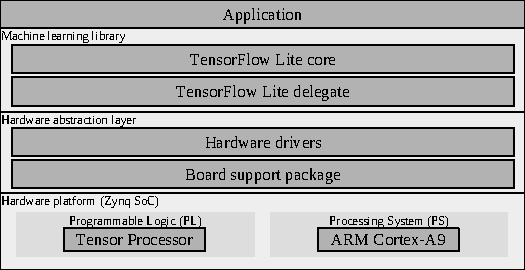
\includegraphics[width=0.5\textwidth]{../figures/sw_stack.pdf}
	\caption{Base embedded software architecture.}
	\label{fig:sw_stack}
\end{figure}
\subsection{Embedded software architecture}
The software architecture is a layered object-oriented application framework written in C++, see \fig{fig:sw_stack}. The main characteristics o the software layers are as follows:
\begin{itemize}
	\item \emph{Application}: As the highest level of abstraction, this layer implements the embedded application logic with the ML library.
	\item \emph{Machine learning library}: This layer consist of TensorFlow Lite micro. This offers a comprehensive high level API that allows ML inference. This provides delegate interfaces for custom hardware accelerators.
	\item \emph{Hardware abstraction layer}: This layer consist of the hardware drivers to handle initialization and runtime operation of the TP and DMA.
\end{itemize}